% $Header$

\documentclass[aspectratio=1610]{beamer}

\mode<presentation>
{%
  \usetheme{Boadilla}
}


\usepackage[english]{babel}
\usepackage[utf8]{inputenc}
\usepackage[T1]{fontenc}

\usepackage{%
    animate,
    graphicx,
    varwidth,
    tcolorbox,
    clrscode3e,
    tikz,
    mathtools,
    forest,
}
\usetikzlibrary{overlay-beamer-styles, positioning, matrix}

\tikzset{%
    node/.style={circle,thick,draw},
    label/.style={fill=white,circle,font=\small},
    every edge/.style={draw,very thick},
}

\graphicspath{{../../imgs/graphs/}}

% alert a whole line (especially for algorithms)
\newcommand{\alertline}{%
\usebeamercolor[fg]{normal text}%
\only{\usebeamercolor[fg]{alerted text}}}

% floor command
\newcommand{\floor}[1]{\left\lfloor #1 \right\rfloor}

\title[ALG25 - Lecture 8]
{Elementære Grafalgoritmer}

\subtitle
{Algorithms and Datastructures, F25, Lecture 8}

\author[Andreas H. Høeg-Petersen]
{Andreas Holck Høeg-Petersen}

\institute[AAU]{%
  Department of Computer Science\\
  Aalborg University
}

\date {\today}

\pgfdeclareimage[height=0.5cm]{university-logo}{../../imgs/aau-logo}
\logo{%
    \begin{tikzpicture}[overlay,remember picture]
        \node[left=0.2cm] at (current page.30){\pgfuseimage{university-logo}};
    \end{tikzpicture}
}

\AtBeginSection[]
{%
  \begin{frame}<beamer>{Outline}
    \tableofcontents[currentsection,currentsubsection]
  \end{frame}
}

\begin{document}

\begin{frame}
  \titlepage
\end{frame}

\begin{frame}{Opdateringer}{}
    \begin{itemize}[<+->]
        \small
        \item Tak for mange fine afleveringer! De vil blive behandlet\ldots i
            løbet af og efter påsken
        \item I dag blev mine nye slides kun 90\% færdige - så der er lige et
            blast from the past i slutningen af forelæsningen 
    \end{itemize}
\end{frame}


\begin{frame}{Outline}
  \tableofcontents
\end{frame}

\section{Grafer og deres repræsentationer}

\begin{frame}{Grafer}{Hvad og hvorfor?}
    En graf er en måde at repræsentere objekter og deres interne relationer.

    \begin{columns}
        \column{.7\textwidth}
        \begin{itemize}[<+(1)->]
            \small
            \item Ligesom træer, har grafer \alert{knuder} (verticies/nodes),
                der er forbundet af \alert{kanter} (edges)
            \item Modsat træer, er der ikke nødvendigvis nogen naturlig rækkefølge
                at læse grafen i (på?)
            \item Vi specificerer en graf $G = (V,E)$, hvor $V$ er mængden af
                knuder og $E \subset V \times V$ er mængden af kanter
            \item Grafer er en \textit{ekstrem} fleksibel datastruktur til at
                modellere problemer med
                \begin{itemize}
                    \footnotesize
                    \item Dependency trees
                    \item Tidsserier
                    \item Stifinding i netværk eller kort
                    \item Internettet er en stor graf --- det samme er sociale
                        netværk
                    \item Kan modellerer sandsynlighedsdistributioner (Bayesian
                        networks)
                    \item Neurale netværk er basically grafer og trænes ved at
                        konstruere en computational graph for gradienterne
                        (backpropagation)
                    \item \ldots og meget, meget mere
                \end{itemize}
        \end{itemize}
    
        \column{.3\textwidth}
        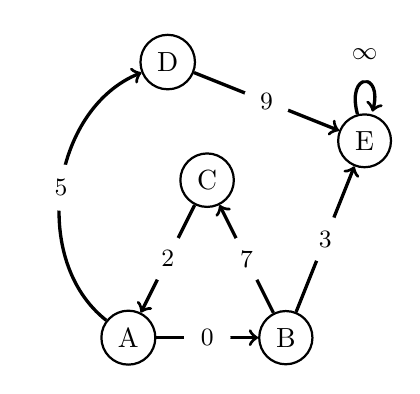
\begin{tikzpicture}
            \node[node] (A) at (0,0) {A};
            \node[node] (B) at (2,0) {B};
            \node[node] (C) at (1,2) {C};
            \node[node] (D) at (0.5,3.5) {D};
            \node[node] (E) at (3,2.5) {E};

            \path [->] (A) edge[bend left=60] node[label] {$5$} (D);
            \path [->] (C) edge node[label] {$2$} (A);
            \path [->] (B) edge node[label] {$7$} (C);
            \path [->] (B) edge node[label] {$3$} (E);
            \path [->] (D) edge node[label] {$9$} (E);
            \path [->] (A) edge node[label] {$0$} (B);
            \path [->] (E) edge[loop above] node[label] {$\infty$} ();
        \end{tikzpicture}
    \end{columns}

\end{frame}


\begin{frame}{Grafer}{Orienterede og ikke-orienterede}
    Grafer kommer overordnet set i to varianter:

    \begin{columns}[t]
        \column{.5\textwidth}<2->
        \small
        \begin{itemize}
            \item I \alert{orienterede} (directed) grafer har hver kant en retning
            \item En kant $(u,v) \in E$ er en kant, der går \alert{fra} knude
                $u$ \alert{til} knude $v$
        \end{itemize}

        \begin{center}
            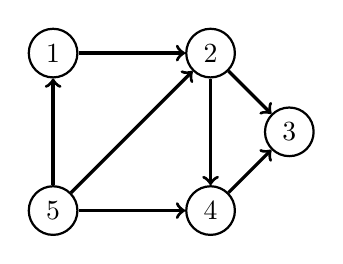
\begin{tikzpicture}
                \node[node] (5) at (0,0) {5};
                \node[node] (1) at (0,2) {1};
                \node[node] (4) at (2,0) {4};
                \node[node] (2) at (2,2) {2};
                \node[node] (3) at (3,1) {3};

                \path [->] (5) edge (1);
                \path [->] (5) edge (2);
                \path [->] (5) edge (4);
                \path [->] (2) edge (4);
                \path [->] (1) edge (2);
                \path [->] (2) edge (3);
                \path [->] (4) edge (3);
            \end{tikzpicture}
        \end{center}
        \vspace{-\abovedisplayskip}
        \begin{alignat*}{2}
            V&= \{&& 5,1,2,4,3\} \\
            E&= \{&&(5,1),(5,2),(5,4),(1,2), \\ & &&(2,3),(2,4),(3,4) \}
        \end{alignat*}
    
        \column{.5\textwidth}<3->
        \small
        \begin{itemize}
            \item I \alert{ikke-orienterede} (undirected) grafer har en kant
                ${u,v} \in E$ ikke en retning, men forbinder $u$ og $v$ i begge
                retninger
            \item Ikke-orienterede grafer er en special case af orienterede
                grafer
        \end{itemize}

        \begin{center}
            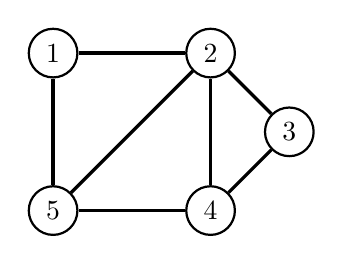
\begin{tikzpicture}
                \node[node] (5) at (0,0) {5};
                \node[node] (1) at (0,2) {1};
                \node[node] (4) at (2,0) {4};
                \node[node] (2) at (2,2) {2};
                \node[node] (3) at (3,1) {3};

                \path [-] (5) edge (1);
                \path [-] (5) edge (2);
                \path [-] (5) edge (4);
                \path [-] (2) edge (4);
                \path [-] (1) edge (2);
                \path [-] (2) edge (3);
                \path [-] (4) edge (3);
            \end{tikzpicture}
        \end{center}
        \vspace{-\abovedisplayskip}
        \begin{alignat*}{2}
            V&= \{&& 5,1,2,4,3\} \\
            E&= \{&&\{5,1\},\{5,2\},\{5,4\},\{1,2\}, \\ & &&\{2,3\},\{2,4\},\{3,4\} \}
        \end{alignat*}

    \end{columns}
\end{frame}

\begin{frame}{Grafer}{Flere detaljer}
    \begin{columns}
        \column{.6\textwidth}
        \begin{itemize}[<+(1)->]
            \small
            \item Når vi analyserer grafer, angiver vi typisk kompleksiteten som
                en funktion af både $|V|$ og $|E|$
            \item Hvor mange kanter ($|E|$) kan der maksimalt være i en graf med
                $|V|$ knuder?
                \begin{itemize}
                    \item For en ikke-orienteret graf, $|E| = \binom{|V|}{2} =
                        \frac{|V|(|V|-1)}{2} = O(|V|^2)$
                    \item For en orienteret graf, $|E| = |V|(|V|-1) = O(|V|^2)$
                \end{itemize}
            \item Hvis $|E|$ er meget mindre end $|V|^2$ siger vi, at grafen er
                \alert{sparse}
            \item Hvis $|E|$ er tæt på $|V|^2$ siger vi, at grafen er
                \alert{dense}
            \item Vi kan også have at gøre med \alert{vægtede} grafer
                \begin{itemize}
                    \item Her antager vi en \alert{weight function} $w: E
                        \rightarrow \mathbb{R}$, hvor $w(u,v)$ giver vægten af
                        kanten fra $u$ til $v$
                \end{itemize}
        \end{itemize}
    
        \column{.4\textwidth}

        \begin{center}
            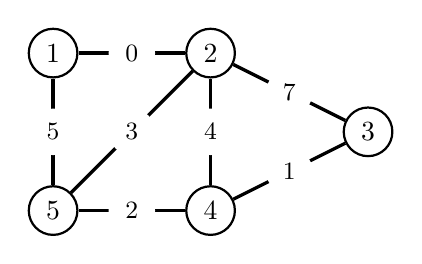
\begin{tikzpicture}
                \node[node] (5) at (0,0) {5};
                \node[node] (1) at (0,2) {1};
                \node[node] (4) at (2,0) {4};
                \node[node] (2) at (2,2) {2};
                \node[node] (3) at (4,1) {3};

                \path [-] (5) edge node[label,visible on= <8->] {$5$} (1);
                \path [-] (5) edge node[label,visible on= <8->] {$3$} (2);
                \path [-] (5) edge node[label,visible on= <8->] {$2$} (4);
                \path [-] (2) edge node[label,visible on= <8->] {$4$} (4);
                \path [-] (1) edge node[label,visible on= <8->] {$0$} (2);
                \path [-] (2) edge node[label,visible on= <8->] {$7$} (3);
                \path [-] (4) edge node[label,visible on= <8->] {$1$} (3);
            \end{tikzpicture}

        \end{center}
        \begin{alignat*}{2}
            V&= \{&& 5,1,2,4,3\} \\
            E&= \{&&\{5,1\},\{5,2\},\{5,4\},\{1,2\}, \\
             &    &&\{2,3\},\{2,4\},\{3,4\} \} 
        \end{alignat*}

    \end{columns}
\end{frame}


\begin{frame}{Repræsentation af grafer}{Adjacency matrix}
    Vi skal se på to måder at repræsentere grafer på:

    \begin{columns}
        \column{.6\textwidth}
        \begin{itemize}[<+(1)->]
            \item For en graf $G = (V,E)$ er en \alert{adjacency matrix} en
                matrix (duh!) med størrelse $|V|^2$
            \item Hvert element i matricen $A=(a_{ij})$ defineres således at
                \begin{equation*}
                    a_{ij} =
                    \begin{cases}
                        1 & \text{if } (i,j) \in E \\
                        0 & \text{otherwise}
                    \end{cases}
                \end{equation*}
            \item Nemt når vi skal repræsentere \alert{vægtede} grafer --- så
                lader vi bare $a_{ij} = w(i,j)$ hvis $(i,j) \in E$
            \item Hvor meget plads bruger dette? \uncover<6->{$O(|V|^2)$}
            \item Derfor mest oplagt hvis grafen er dense
        \end{itemize}
    
        \column{.4\textwidth}
        \begin{center}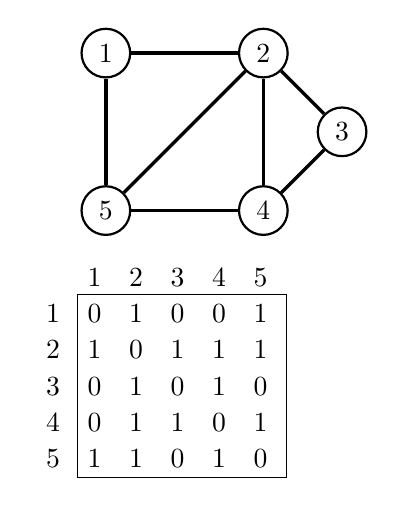
\begin{tikzpicture}
            \node[node] (5) at (0,0) {5};
            \node[node] (1) at (0,2) {1};
            \node[node] (4) at (2,0) {4};
            \node[node] (2) at (2,2) {2};
            \node[node] (3) at (3,1) {3};

            \matrix (m) [
            align=center,
            matrix anchor=west,
            ampersand replacement=\&,
            matrix of math nodes,
            column sep=0,row sep=0,
            every column/.style={nodes={align=center}},
            ] at (-1,-2) {%
                \& 1 \& 2 \& 3 \& 4 \& 5 \\
                1 \& 0 \& 1 \& 0 \& 0 \& 1 \\
                2 \& 1 \& 0 \& 1 \& 1 \& 1 \\
                3 \& 0 \& 1 \& 0 \& 1 \& 0 \\
                4 \& 0 \& 1 \& 1 \& 0 \& 1 \\
                5 \& 1 \& 1 \& 0 \& 1 \& 0 \\
            };
        \draw (m-2-2.north west) rectangle (m-6-6.south east);
        \path [-] (5) edge (1);
        \path [-] (5) edge (2);
        \path [-] (5) edge (4);
        \path [-] (2) edge (4);
        \path [-] (1) edge (2);
        \path [-] (2) edge (3);
        \path [-] (4) edge (3);
    \end{tikzpicture}\end{center}
    \end{columns}
\end{frame}


\begin{frame}{Repræsentation af grafter}{Adjacency lists}
    Den anden måde er ved brug af \alert{adjacency lists}:

    \begin{columns}
        \column{.6\textwidth}
        \begin{itemize}[<+(1)->]
            \item En adjacency lists for en graf $G = (V,E)$ består af et array
                (eller en hash-table) $\id{Adj}[1:|V|]$
            \item For hver knude $u \in V$ har vi en liste $\id{Adj}[u]$, som
                indeholder alle knuder $v$ hvor $\{u,v\} \in E$
            \item Hvor meget plads bruger dette?
                \begin{itemize}
                    \item $O(|V| + |E|)$
                \end{itemize}
            \item Bedre eller værre end adjacency matrix?
                \begin{itemize}
                    \item Meget bedre hvis grafen er sparse
                \end{itemize}
        \end{itemize}

        \column{.4\textwidth}
        \begin{center}
            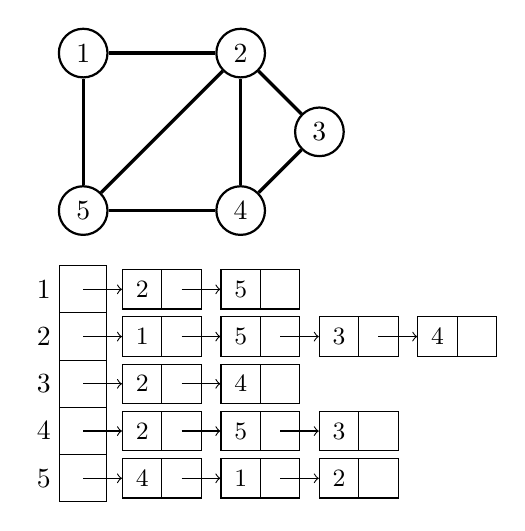
\begin{tikzpicture}[
                lnode/.style={draw,minimum size=.5cm,font=\small},
                snode/.style={draw,minimum size=.6cm},
                ]
            \node[node] (5) at (0,6) {5};
            \node[node] (1) at (0,8) {1};
            \node[node] (4) at (2,6) {4};
            \node[node] (2) at (2,8) {2};
            \node[node] (3) at (3,7) {3};
            %
            \path [-] (5) edge (1);
            \path [-] (5) edge (2);
            \path [-] (5) edge (4);
            \path [-] (2) edge (4);
            \path [-] (1) edge (2);
            \path [-] (2) edge (3);
            \path [-] (4) edge (3);
            %
                \node[snode] (10) at (0,    5) {};
                \node[lnode] (11) at (0.75, 5) {2};
                \node[lnode] (12) at (1.25, 5) {};
                \node[lnode] (13) at (2.00, 5) {5};
                \node[lnode] (14) at (2.50, 5) {};
                \node[draw=none] (1) at (-0.50,5) {1};
                %
                \draw [->] (10.center) -- (11);
                \draw [->] (12.center) -- (13);
                %
                \node[snode] (20) at (0,    4.40) {};
                \node[lnode] (21) at (0.75, 4.40) {1};
                \node[lnode] (22) at (1.25, 4.40) {};
                \node[lnode] (23) at (2.00, 4.40) {5};
                \node[lnode] (24) at (2.50, 4.40) {};
                \node[lnode] (25) at (3.25, 4.40) {3};
                \node[lnode] (26) at (3.75, 4.40) {};
                \node[lnode] (27) at (4.50, 4.40) {4};
                \node[lnode] (28) at (5.00, 4.40) {};
                \node[draw=none] (2) at (-0.50,4.40) {2};
                %
                \draw [->] (20.center) -- (21);
                \draw [->] (22.center) -- (23);
                \draw [->] (24.center) -- (25);
                \draw [->] (26.center) -- (27);
                %
                \node[snode] (30) at (0,    3.8) {};
                \node[lnode] (31) at (0.75, 3.8) {2};
                \node[lnode] (32) at (1.25, 3.8) {};
                \node[lnode] (33) at (2.00, 3.8) {4};
                \node[lnode] (34) at (2.50, 3.8) {};
                \node[draw=none] (3) at (-0.50,3.8) {3};
                %
                \draw [->] (30.center) -- (31);
                \draw [->] (32.center) -- (33);
                %
                \node[snode] (40) at (0,    3.2) {};
                \node[lnode] (41) at (0.75, 3.2) {2};
                \node[lnode] (42) at (1.25, 3.2) {};
                \node[lnode] (43) at (2.00, 3.2) {5};
                \node[lnode] (44) at (2.50, 3.2) {};
                \node[lnode] (45) at (3.25, 3.2) {3};
                \node[lnode] (46) at (3.75, 3.2) {};
                \node[draw=none] (4) at (-0.50,3.2) {4};
                %
                \draw [->] (40.center) -- (41);
                \draw [->] (42.center) -- (43);
                \draw [->] (44.center) -- (45);
                %
                \node[snode] (50) at (0,    2.6) {};
                \node[lnode] (51) at (0.75, 2.6) {4};
                \node[lnode] (52) at (1.25, 2.6) {};
                \node[lnode] (53) at (2.00, 2.6) {1};
                \node[lnode] (54) at (2.50, 2.6) {};
                \node[lnode] (55) at (3.25, 2.6) {2};
                \node[lnode] (56) at (3.75, 2.6) {};
                \node[draw=none] (5) at (-0.50,2.6) {5};
                %
                \draw [->] (50.center) -- (51);
                \draw [->] (52.center) -- (53);
                \draw [->] (54.center) -- (55);
            \end{tikzpicture}
        \end{center}
    \end{columns}
\end{frame}


\section{Breadth-first search}

\begin{frame}{Søgning i grafer}{Breadth-first search}
    Vi ser nu på to fundamentale måder at søge i en graf på.

    \begin{itemize}[<+(1)->]
        \item \alert{Breadth-first search} (BFS) søger, som navnet indikerer, i
            `bredden' først
        \item Givet en graf $G = (V,E)$ og en start-knude $s \in V$ finder BFS
            (afstanden på) den korteste sti fra $s$ til alle andre knuder i $G$
            (der kan nåes fra $s$)\footnote{%
                Gælder kun for ikke-vægtede grafer
            }
        \item Undervejs besøges \alert{alle} knuder i $V$, der kan nåes fra $s$,
            og på hver knude $v$, som vi kommer til fra $u$, noterer vi dens
            \alert{predecessor} $\attrib{v}{\pi} = u$
        \item Som artefakt får vi en \alert{predecessor subgraph} af $G$ i form
            af $G_{\pi} = (V_{\pi},E_{\pi})$
            \begin{itemize}
                \item Hvor
                    \begin{align*}
                        V_{\pi}&= \{v \in V : \attrib{v}{\pi} \neq \const{NIL}
                        \} \cup \{s\} \\
                            E_{\pi}&= \{(\attrib{v}{\pi},v) : v \in V_{\pi} -
                            \{s\}\}
                    \end{align*}
                \item Denne subgraf kalder vi også et \alert{breadth-first tree}
                    $T$ med rod i $s$ og hvor alle stier fra $s$ til enhver
                    anden knude $v \in T$ svarer til den korteste sti fra $s$
                    til $v$ i $G$
            \end{itemize}
        \item Fungerer både på orienterede og ikke-orienterede grafer
    \end{itemize}
\end{frame}

\begin{frame}<1-10>{Breadth-first search}{Eksempel}
    \begin{columns}
        \column{.5\textwidth}
        \begin{center}\begin{tikzpicture}[
            scale=0.75,
            every node/.style={draw,circle,minimum size=.8cm,align=center},
            white/.style={fill=white!50},
            gray/.style={fill=gray!50, text=black},
            black/.style={fill=black, text=white, font=\bfseries},
            switch/.style={alt={####1{}{semithick}}},
            ]
            \node[draw=none] (t) at (0,-0.75) {$t$};
            \node<-2> [white] (t1) at (0,0) {$\infty$};
            \node<3-5>[gray]  (t2) at (0,0) {2};
            \node<6-> [black] (t3) at (0,0) {2};
            %
            \node[draw=none] (u) at (2,-1.75) {$u$};
            \node<1>  [white] (u1) at (2,-1) {$\infty$};
            \node<2-3>[gray]  (u2) at (2,-1) {1};
            \node<4-> [black] (u3) at (2,-1) {1};
            %
            \node[draw=none] (y) at (4,-0.75) {$y$};
            \node<-3> [white] (y1) at (4,0) {$\infty$};
            \node<4-8>[gray]  (y2) at (4,0) {2};
            \node<8-> [black] (y3) at (4,0) {2};
            %
            \node[draw=none] (s) at (2,1.75) {$s$};
            \node<1>  [gray]  (s1) at (2,1) {0};
            \node<2-> [black] (s2) at (2,1) {0};
            %
            \node[draw=none] (r) at (0.5,2.75) {$r$};
            \node<-1> [white] (r1) at (0.5,2) {$\infty$};
            \node<2-2>[gray]  (r2) at (0.5,2) {1};
            \node<3-> [black] (r3) at (0.5,2) {1};
            %
            \node[draw=none] (v) at (3.5,2.75) {$v$};
            \node<-1> [white] (v1) at (3.5,2) {$\infty$};
            \node<2-4>[gray]  (v2) at (3.5,2) {1};
            \node<5-> [black] (v3) at (3.5,2) {1};
            %
            \node[draw=none] (w) at (2,4.75) {$w$};
            \node<-2> [white] (w1) at (2,4) {$\infty$};
            \node<3-6>[gray]  (w2) at (2,4) {2};
            \node<7-> [black] (w3) at (2,4) {2};
            %
            \node[draw=none] (x) at (6,4.75) {$x$};
            \node<-6> [white] (x1) at (6,4) {$\infty$};
            \node<7-8>[gray]  (x2) at (6,4) {3};
            \node<9-> [black] (x3) at (6,4) {3};
            %
            \node[draw=none] (z) at (7,2.75) {$z$};
            \node<-6> [white] (z1) at (7,2) {$\infty$};
            \node<7-9>[gray]  (z2) at (7,2) {3};
            \node<10->[black] (z3) at (7,2) {3};
            %
            \draw [-] (s1) edge[switch=<2->] (r1);
            \draw [-] (s1) edge[switch=<2->] (v1);
            \draw [-] (s1) edge[switch=<2->] (u1);
            \draw [-] (t1) edge[switch=<3->] (r1);
            \draw [-] (w1) edge[switch=<3->] (r1);
            \draw [-] (u1) edge[switch=<4->] (y1);
            \draw [-] (w1) edge[switch=<7->] (x1);
            \draw [-] (w1) edge[switch=<7->] (z1);
            \draw [-] (t1) edge[semithick] (u1);
            \draw [-] (y1) edge[semithick] (v1);
            \draw [-] (y1) edge[semithick] (x1);
            \draw [-] (v1) edge[semithick] (w1);
        \end{tikzpicture}

        $Q = \langle 
        \only<1>{s}\only<2>{r}\only<3>{u}\only<4>{v}\only<5>{t}\only<6>{w}\only<7>{y}\only<8>{x}\only<9>{z}\only<2-8>{,}
        \only<2>{u}\only<3>{v}\only<4>{t}\only<5>{w}\only<6>{y}\only<7>{x}\only<8>{z}\only<2-5,7>{,}
        \only<2>{v}\only<3>{t}\only<4>{w}\only<5>{y}\only<7>{z}\only<3,4>{,}
        \only<3>{w}\only<4>{y}
        \rangle$

    \end{center}    

        \column{.5\textwidth}
        \begin{itemize}
            \item<1-> Vi starter fra $s$ og antager, at alle andre knuder er uendeligt
                langt væk fra $s$
            \item<2-> Så gemmer vi alle naboer til $s$ i en kø $Q$ og noterer, hvor
                langt væk de var
            \item<3-> Så dequeuer vi det første element i $Q$ (som her er $r$),
                tilføjer dets naboer til $Q$ og noterer afstanden til $s$
            \item<4-> Dette fortsætter vi med, og fordi vi bruger en queue tager vi
                alt i en breadth-first rækkefølge
            \item<5-> Da vi allerede har besøgt alle $v$'s naboer, så skal vi
                bare markere den som færdig
            \item<10-> Når alle knuder er færdigbehandlet, udgør de fede kanter
                hele breadth-first træet $T$
        \end{itemize}
    \end{columns}

\end{frame}

\begin{frame}{Breadth-first search}{Pseudo-kode}
    \begin{columns}
        \column{.5\textwidth}
        \begin{block}{$\proc{BFS}(G,s)$}
            \footnotesize
        
            \vspace{-\abovedisplayskip}
            \begin{codebox}
                \li \alertline<2,10>\For each vertex $u \in G.V - \{s\}$
                    \Do
                \li     \alertline<2>$\attrib{u}{color} \gets \const{WHITE}$ 
                \li     \alertline<2>$\attrib{u}{d} \gets \infty$ 
                \li     \alertline<2>$\attrib{u}{\pi} \gets \const{NIL}$ 
                    \End
                \li \alertline<3>$\attrib{s}{color} \gets \const{GRAY}$ 
                \li \alertline<3>$\attrib{s}{d} \gets 0$ 
                \li \alertline<3>$\attrib{s}{\pi} \gets \const{NIL}$ 
                \li \alertline<3>$Q \gets \emptyset$ 
                \li \alertline<3,11>$\proc{Enqueue}(Q,s)$
                \li \alertline<4>\While $Q \neq \emptyset$
                    \Do
                \li     \alertline<4>$u \gets \proc{Dequeue}(Q)$
                \li     \alertline<5,12>\For each vertex $v \in \attrib{G}{\id{Adj}[u]}$ 
                        \Do
                \li         \alertline<5,11>\If $\attrib{v}{color} \isequal \const{WHITE}$ 
                            \Then
                \li             \alertline<6>$\attrib{v}{color} \gets \const{GRAY}$ 
                \li             \alertline<6>$\attrib{v}{d} \gets \attrib{u}{d} + 1$ 
                \li             \alertline<6>$\attrib{v}{\pi} \gets u$ 
                \li             \alertline<6,11>$\proc{Enqueue}(Q,v)$
                            \End
                        \End
                \li     \alertline<7>$\attrib{u}{color} \gets \const{BLACK}$ 
                    \End


            \end{codebox}
        \end{block}

        \column{.5\textwidth}
        \only<-8>{%
            \begin{itemize}
                \item<2-> Vi annoterer hver knude $u$  med attributterne
                    \begin{itemize}
                        \item $\attrib{u}{color} \in \{ \const{WHITE}, \const{GRAY},
                            \const{BLACK} \}$ 
                        \item $\attrib{u}{d}$ , afstanden fra $s$ 
                        \item $\attrib{u}{\pi}$ , $u$'s mor i breadth-first træet
                    \end{itemize}
                \item<3-> Så sætter vi $s$ til at være grå, angiver dens afstand (til
                    den selv) som 0 og indsætter den som første og hidtil eneste
                    element i $Q$
                \item<4-> Sålænge $Q$ ikke er tom, så dequeuer vi det forreste
                    element $u$
                \item<5-> Herefter løber vi alle $u$'s naboer igennem, og hvis de er
                    hvide, så har vi endnu ikke behandlet dem
                \item<6-> I så fald maler vi dem grå, sætter afstand og mor og
                    tilføjer dem til $Q$
                \item<7-> Til sidst maler vi $u$ sort
            \end{itemize}
        }

        \only<9->{%
            \begin{itemize}[<+(8)->]
                \item Hvad er kompleksiteten?
                \item Initialiseringen løber gennem alle knuder, ergo $O(|V|)$
                \item Efter initialisering gøres en knude aldrig hvid igen --- ergo,
                    enqueues og dequeues hver knude højst 1 gang, så $O(|V|)$
                \item Dermed bliver hver adjacency liste også kun scannet 1 gang
                \item Den totale længde af alle adjacency lister er $\Theta(|E|)$
                \item Altså bliver den samlede køretid af BFS $O(|V| + |E|)$
            \end{itemize}
        }
    \end{columns}
\end{frame}

\section{Exercises}

\begin{frame}{Exercises}{Super fedt! <3}

    På Moodle! Go! Fungerer det fint?

    \begin{figure}[h]
        \centering
        
\includegraphics[width=0.8\textwidth]{../exercises}
    \end{figure}

\end{frame}

\section{Depth-first search}

\begin{frame}{Depth-first search}{Nu går vi dybere!}
    Den anden søgemetode hedder \alert{depth-first search} (DFS).

    \begin{itemize}[<+(1)->]
        \item Her tager vi ikke udgangspunkt i en bestemt start-knude, men i
            stedet går vi alle knuder i grafen igennem
        \item I stedet for at udfdorske hele `niveauer' i grafen først, så
            følger vi stien fra en knude til dens `dybeste' efterkommer inden,
            at vi går videre til naboer
        \item I stedet for et `breadth-first \alert{tree}', så får vi med DFS en
            `depth-first \alert{forest}' (der kan være flere rødder, som ikke er
            forbundne)
            \begin{itemize}
                \item Dette er en \alert{predecessor subgraph} $G_{\pi} =
                    (V,E_{\pi})$ hvor
                     \[
                         E_{\pi} = \{(\attrib{v}{\pi}, v) : v \in V \text{and }
                         \attrib{v}{\pi} \neq \const{NIL} \}
                    \] 
            \end{itemize}
    \end{itemize}
\end{frame}


\begin{frame}{Depth-first search}{Algoritme}

    \begin{columns}
        \column{.6\textwidth}
        \begin{itemize}
            \item<2-> Proceduren $\proc{DFS}(G)$ initialiserer alle knuder og
                starter `timeren'
            \item<3-> Herefter tager den knuderne en af gangen og kalder
                sub-proceduren $\proc{DFS-Visit}$ på dem (hvis de stadig er
                hvide)
            \item<4-> I $\proc{DFS-Visit}$ noterer vi, hvornår vi `opdagede' $u$
                ved at sætte $\attrib{u}{d} = \id{time}$
            \item<5-> Herefter tager vi hver nabo $v$ til $u$, sætter
                $\attrib{v}{\pi}$ og kalder $\proc{DFS-Visit}$ rekursivt på $v$
                (såfremt den er hvid)
            \item<6-> Til sidst noterer vi på $u$, hvornår vi færdiggjorde den
                ($\attrib{u}{f}$) og maler den sort
        \end{itemize}
        
    
        \column{.4\textwidth}
        \footnotesize
        \begin{block}{}
        
            \vspace{-1.5\abovedisplayskip}
            \begin{codebox}
                \Procname{$\proc{DFS}(G)$}
                \li \alertline<2>\For each vertex $u \in G.V$ \Do
                \li     \alertline<2>$\attrib{u}{color} \gets \const{WHITE}$ 
                \li     \alertline<2>$\attrib{u}{\pi} \gets \const{NIL}$ 
                    \End
                \li \alertline<2>$time \gets 0$ 
                \li \alertline<3>\For each vertex $u \in G.V$  \Do
                \li     \alertline<3>\If $\attrib{u}{color} \isequal \const{WHITE}$ \Then
                \li         \alertline<3>$\proc{DFS-Visit}(G,u)$
                        \End
                    \End
            \end{codebox}

            \vspace{-2\abovedisplayskip}
            \begin{codebox}
                \Procname{$\proc{DFS-Visit}(G,u)$}
                \li \alertline<4>$\id{time} \gets \id{time} + 1$ 
                \li \alertline<4>$\attrib{u}{d} \gets time$ 
                \li \alertline<4>$\attrib{u}{color} \gets \const{GRAY}$ 
                \li \alertline<5>\For each vertex $v \in \attrib{G}{\id{Adj}[u]}$ \Do
                \li     \alertline<5>\If $\attrib{v}{color} \isequal \const{WHITE}$ \Then
                \li         \alertline<5>$\attrib{v}{\pi} \gets u$ 
                \li         \alertline<5>$\proc{DFS-Visit}(G,v)$
                        \End
                    \End
                \li \alertline<6>$\id{time} \gets \id{time} + 1$ 
                \li \alertline<6>$\attrib{u}{f} \gets \id{time}$ 
                \li \alertline<6>$\attrib{u}{color} \gets \const{BLACK}$ 
            \end{codebox}
        \end{block}
    \end{columns}
\end{frame}

\begin{frame}<1-20>{Depth-first search}{Eksempel}
    \begin{columns}
        \column{.65\textwidth}
        \begin{tikzpicture}[
            every node/.style={draw=none},
            switch/.style={alt={####1{opacity=1}{opacity=.5}}},
            ]
            \node[switch=<2>] at (0,  4.5)
                {\includegraphics<2->[width=.24\columnwidth]{dfs-a}};
            \node[switch=<3>] at (2.5,4.5)
                {\includegraphics<3->[width=.24\columnwidth]{dfs-b}};
            \node[switch=<4>] at (5,  4.5)  {\includegraphics<4->[width=.24\columnwidth]{dfs-c}};
            \node[switch=<5>] at (7.5,4.5)  {\includegraphics<5->[width=.24\columnwidth]{dfs-d}};
            \node[switch=<6>] at (0,  3)    {\includegraphics<6->[width=.24\columnwidth]{dfs-e}};
            \node[switch=<7>] at (2.5,3)    {\includegraphics<7->[width=.24\columnwidth]{dfs-f}};
            \node[switch=<8>] at (5,  3)    {\includegraphics<8->[width=.24\columnwidth]{dfs-g}};
            \node[switch=<9>] at (7.5,3)    {\includegraphics<9->[width=.24\columnwidth]{dfs-h}};
            \node[switch=<10>] at (0,  1.5) {\includegraphics<10->[width=.24\columnwidth]{dfs-i}};
            \node[switch=<11>] at (2.5,1.5) {\includegraphics<11->[width=.24\columnwidth]{dfs-j}};
            \node[switch=<12>] at (5,  1.5) {\includegraphics<12->[width=.24\columnwidth]{dfs-k}};
            \node[switch=<13>] at (7.5,1.5) {\includegraphics<13->[width=.24\columnwidth]{dfs-l}};
            \node[switch=<14>] at (0,  0)   {\includegraphics<14->[width=.24\columnwidth]{dfs-m}};
            \node[switch=<15>] at (2.5,0)   {\includegraphics<15->[width=.24\columnwidth]{dfs-n}};
            \node[switch=<16>] at (5,  0)   {\includegraphics<16->[width=.24\columnwidth]{dfs-o}};
            \node[switch=<17>] at (7.5,0)   {\includegraphics<17->[width=.24\columnwidth]{dfs-p}};
        \end{tikzpicture}
        
        \column{.35\textwidth}
        \footnotesize
        \begin{block}{}
        
            \vspace{-1.5\abovedisplayskip}
            \begin{codebox}
                \Procname{$\proc{DFS}(G)$}
                \li \For each vertex $u \in G.V$ \Do
                \li     $\attrib{u}{color} \gets \const{WHITE}$ 
                \li     $\attrib{u}{\pi} \gets \const{NIL}$ 
                    \End
                \li $time \gets 0$ 
                \li \For each vertex $u \in G.V$  \Do
                \li     \If $\attrib{u}{color} \isequal \const{WHITE}$ \Then
                \li         $\proc{DFS-Visit}(G,u)$
                        \End
                    \End
            \end{codebox}

            \vspace{-2\abovedisplayskip}
            \begin{codebox}
                \Procname{$\proc{DFS-Visit}(G,u)$}
                \li $\id{time} \gets \id{time} + 1$ 
                \li $\attrib{u}{d} \gets time$ 
                \li $\attrib{u}{color} \gets \const{GRAY}$ 
                \li \For each vertex $v \in \attrib{G}{\id{Adj}[u]}$ \Do
                \li     \If $\attrib{v}{color} \isequal \const{WHITE}$ \Then
                \li         $\attrib{v}{\pi} \gets u$ 
                \li         $\proc{DFS-Visit}(G,v)$
                        \End
                    \End
                \li $\id{time} \gets \id{time} + 1$ 
                \li $\attrib{u}{f} \gets \id{time}$ 
                \li $\attrib{u}{color} \gets \const{BLACK}$ 
            \end{codebox}
        \end{block}

    \end{columns}
\end{frame}

\begin{frame}{Depth-first search}{Analyse}

    \begin{columns}
        \column{.4\textwidth}
        \footnotesize
        \begin{block}{}
        
            \vspace{-1.5\abovedisplayskip}
            \begin{codebox}
                \Procname{$\proc{DFS}(G)$}
                \li \alertline<2>\For each vertex $u \in G.V$ \Do
                \li     \alertline<2>$\attrib{u}{color} \gets \const{WHITE}$ 
                \li     \alertline<2>$\attrib{u}{\pi} \gets \const{NIL}$ 
                    \End
                \li \alertline<2>$time \gets 0$ 
                \li \alertline<3>\For each vertex $u \in G.V$  \Do
                \li     \alertline<3>\If $\attrib{u}{color} \isequal \const{WHITE}$ \Then
                \li         \alertline<3>$\proc{DFS-Visit}(G,u)$
                        \End
                    \End
            \end{codebox}

            \vspace{-2\abovedisplayskip}
            \begin{codebox}
                \Procname{$\proc{DFS-Visit}(G,u)$}
                \li \alertline<4>$\id{time} \gets \id{time} + 1$ 
                \li \alertline<4>$\attrib{u}{d} \gets time$ 
                \li \alertline<4>$\attrib{u}{color} \gets \const{GRAY}$ 
                \li \alertline<5>\For each vertex $v \in \attrib{G}{\id{Adj}[u]}$ \Do
                \li     \alertline<5>\If $\attrib{v}{color} \isequal \const{WHITE}$ \Then
                \li         \alertline<5>$\attrib{v}{\pi} \gets u$ 
                \li         \alertline<5>$\proc{DFS-Visit}(G,v)$
                        \End
                    \End
                \li \alertline<6>$\id{time} \gets \id{time} + 1$ 
                \li \alertline<6>$\attrib{u}{f} \gets \id{time}$ 
                \li \alertline<6>$\attrib{u}{color} \gets \const{BLACK}$ 
            \end{codebox}
        \end{block}

        \column{.6\textwidth}
        Hvor lang tid tager det?

        \begin{itemize}
            \item<2-> Linie 1-4 i $\proc{DFS}$? \uncover<3->{$O(|V|)$}
            \item<4-> Linie 5-7 i $\proc{DFS}$? \uncover<5->{$O(|V| \cdot
                O(\proc{DFS-Visit}))$}
                \begin{itemize}
                    \item<5-> Hmmm, så en rekursion?
                \end{itemize}
            \item<6-> Linie 1-3 i $\proc{DFS-Visit}$? \uncover<7->{$\Theta(1)$}
            \item<8-> Linie 4-7 i $\proc{DFS-Visit}$? \uncover<9->{$O(|E|)$ og
                så noget med $\proc{DFS-Visit}$ eller hvad?}
            \item<10-> Linie 8-10 er konstante
            \item<11-> Så lander vi i noget ala $O(|V|\cdot |E|)$?
                \begin{itemize}
                    \item<12-> Nej! Strukturen hjælper os:
                    \item<13-> $\proc{DFS-Visit}$ kaldes kun 1 gang pr knude,
                        $O(|V|)$
                    \item<14-> Og vi følger kun hver kant 1 gang, $O(|E|)$
                \end{itemize}
            \item<15-> Så vi lander på velkendte $O(|V| + |E|)$
        \end{itemize}
        
    
    \end{columns}
\end{frame}


\section{Topologisk sortering}

\begin{frame}{Topologisk sortering}{Tilbage til sortering}
    Nu vender vi lige for en kort stund snuden tilbage til sortering og ser på
    en ny sorteringsalgoritme: \alert{Topologisk sortering}

    \begin{itemize}[<+(1)->]
        \item Algoritme til at sortere knuder i en \alert{directed acyclic
            graph} (DAG)
        \item Rækkefølgen kræver bare, at hvis der er en kant fra $u$ til $v$ i
            $G$, så skal $u$ komme før $v$ i output-listen
        \item Dette er smart, f.eks.\ når man skal kompilere software, hvor
            forskellige sub-moduler er afhængige af hinanden
    \end{itemize}
\end{frame}

\begin{frame}{Topologisk sortering}{Pseudo pseudo-kode}
    Algoritmen?

    \begin{block}{$\proc{Topological-Sort}(G)$}
        \footnotesize
    
        \vspace{-\abovedisplayskip}
        \begin{codebox}
            \li call $\proc{DFS}(G)$ to compute finish times $\attrib{v}{f}$ for
            each vertex $v$
            \li as each vertex is finished, insert it onto the front of a linked
            list
            \li \Return the linked list of vertices
        \end{codebox}
    \end{block}

    \begin{itemize}[<+(1)->]
        \item Kompleksitet?
        \item $O(|V| + |E|)$! 
        \item Det gør det til den hurtigeste sorteringsalgoritme, som vi har set
    \end{itemize}

\end{frame}

\begin{frame}{Topologisk sortering}{Eksempel}
    \begin{columns}
        \column{.5\textwidth}
        \begin{figure}[h]
            \centering
            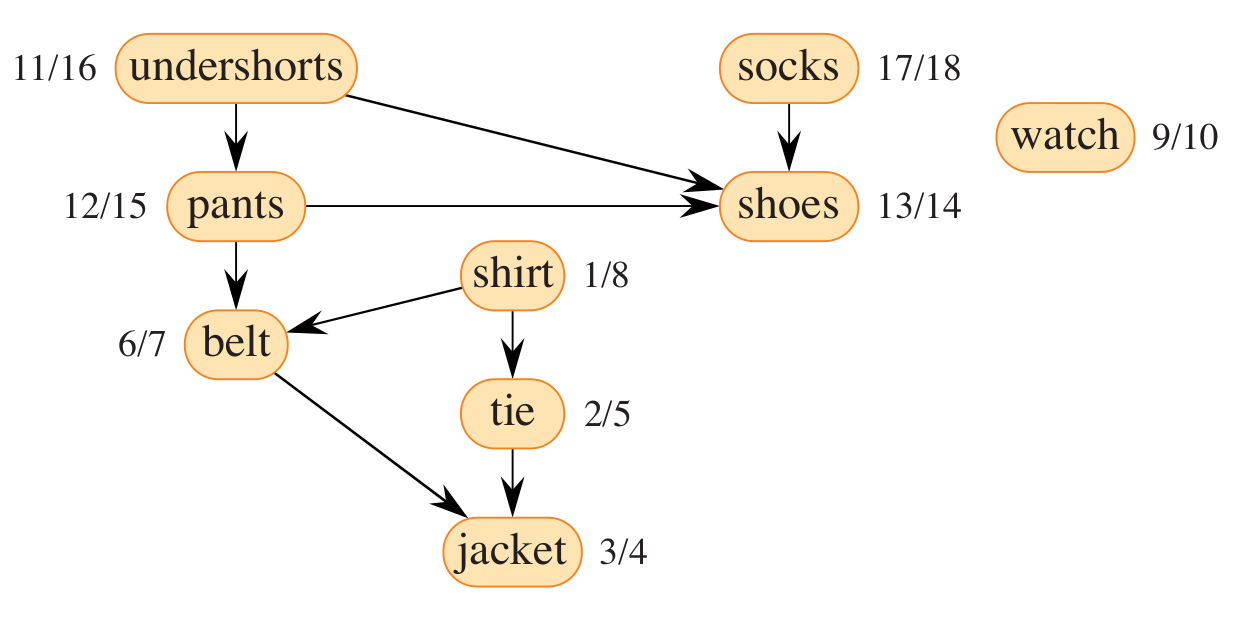
\includegraphics[width=\columnwidth]{topo-dag}
        \end{figure}

        \column{.5\textwidth}
        \begin{block}{$\proc{Topological-Sort}(G)$}
            \footnotesize
        
            \vspace{-\abovedisplayskip}
            \begin{codebox}
                \li call $\proc{DFS}(G)$ to compute
                \Startalign{call $\proc{D}$}
                \>      finish times $\attrib{v}{f}$  for each vertex $x$
                \Stopalign
                \li as each vertex is finished, insert
                \Startalign{as eac}
                \>       it onto the front of a linked list
                \Stopalign
                \li \Return the linked list of vertices
            \end{codebox}
        \end{block}
    \end{columns}

    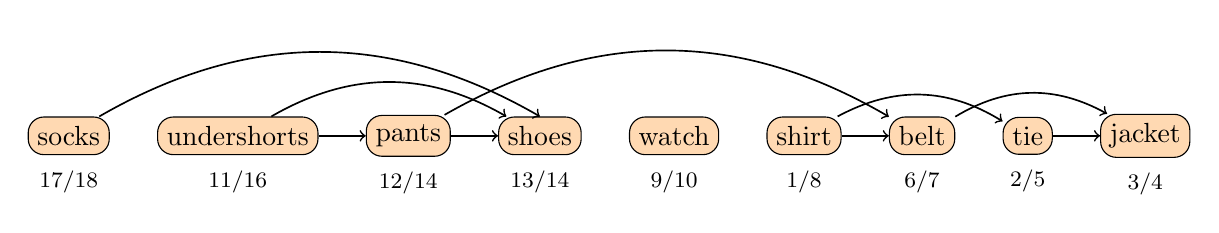
\begin{tikzpicture}[
        every node/.style={%
            draw,
            rounded corners=.2cm,
            fill=orange!30
        },
        every edge/.style={draw,semithick},
        label/.style={draw=none, fill=none, font=\footnotesize},
        node distance=.6cm
        ]
        \node[visible on= <10->] (1) at (0,0)      {socks};
        \node[visible on= <9->]  (2) [right=of 1]  {undershorts};
        \node[visible on= <8->]  (3) [right=of 2]  {pants};
        \node[visible on= <7->]  (4) [right=of 3]  {shoes};
        \node[visible on= <6->]  (5) [right=of 4]  {watch};
        \node[visible on= <5->]  (6) [right=of 5]  {shirt};
        \node[visible on= <4->]  (7) [right=of 6]  {belt};
        \node[visible on= <3->]  (8) [right=of 7]  {tie};
        \node[visible on= <2->]  (9) [right=of 8]  {jacket};
        \node[label,visible on= <2->]  (l9) [below=2pt of 9]  {3/4};
        \node[label,visible on= <3->]  (l8) [below=2pt of 8]  {2/5};
        \node[label,visible on= <4->]  (l7) [below=2pt of 7]  {6/7};
        \node[label,visible on= <5->]  (l6) [below=2pt of 6]  {1/8};
        \node[label,visible on= <6->]  (l5) [below=2pt of 5]  {9/10};
        \node[label,visible on= <7->]  (l4) [below=2pt of 4]  {13/14};
        \node[label,visible on= <8->]  (l3) [below=2pt of 3]  {12/14};
        \node[label,visible on= <9->]  (l2) [below=2pt of 2]  {11/16};
        \node[label,visible on= <10->] (l1) [below=2pt of 1]  {17/18};
        %
        \draw [->] (1) edge[visible on= <10->, bend left=30] (4.north);
        \draw [->] (2) edge[visible on= <9->]                (3);
        \draw [->] (2) edge[visible on= <9->, bend left=30]  (4);
        \draw [->] (3) edge[visible on= <8->]                (4);
        \draw [->] (3) edge[visible on= <8->, bend left=30]  (7);
        \draw [->] (6) edge[visible on= <5->]                (7);
        \draw [->] (6) edge[visible on= <5->, bend left=30]  (8);
        \draw [->] (7) edge[visible on= <4->, bend left=30]  (9);
        \draw [->] (8) edge[visible on= <3->]                (9);
    \end{tikzpicture}
\end{frame}


\begin{frame}{Tak for i dag!}{Flere exercises..}

    Den bedste måde ikke at snyde sig selv på er lave exercises!

    \begin{figure}[h]
        \centering
        
\includegraphics[width=0.8\textwidth]{../exercises}
    \end{figure}

\end{frame}



\end{document}


